\documentclass[12pt,a4paper]{article}
\usepackage[utf8]{inputenc}
\usepackage{amsmath}
\usepackage[brazilian]{babel} % Brazil or not Brazil??
\usepackage{amsfonts}
\usepackage{amssymb}
\usepackage{graphicx}
\usepackage[margin=0.8in]{geometry}


\begin{document}
\title{\vspace{70mm}\Huge Experimento 06a - Calorímetria}
\author{ Giovani Garuffi\qquad\hfill
		\textit {RA: 155559}\protect\\
		João Baraldi\hfill
		\textit{RA: 158044}\protect\\
		Lauro Cruz\hfill
		\textit{RA: 156175}\protect\\
		Lucas Schanner\hfill
		\textit{RA: 156412}\protect\\
		Pedro Stringhini\hfill
		\textit {RA: 156983}								
		}
\maketitle
\newpage
\section{Resumo}


\section{Objetivos}
Este experimento pode ser divido em três partes, cada uma com seus objetivos, que são: traçar um gráfico de calibração de um termopar, calcular a constante de tempo de um calorímetro, e calcular sua capacidade térmica.


\section{Procedimento Experimental e Coleta de Dados}


\subsection{Procedimento}


\subsubsection{Curva de calibração de um termopar}
djng
\begin{figure}
\centering
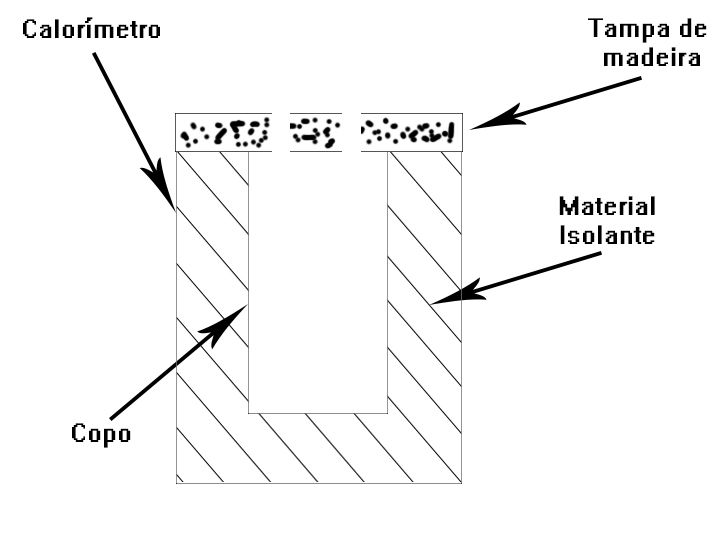
\includegraphics[scale=0.3]{Fig6a1.jpg}
\caption{Calorímetro.}
\label{calorimetro}
\end{figure}

\begin{figure}
\centering
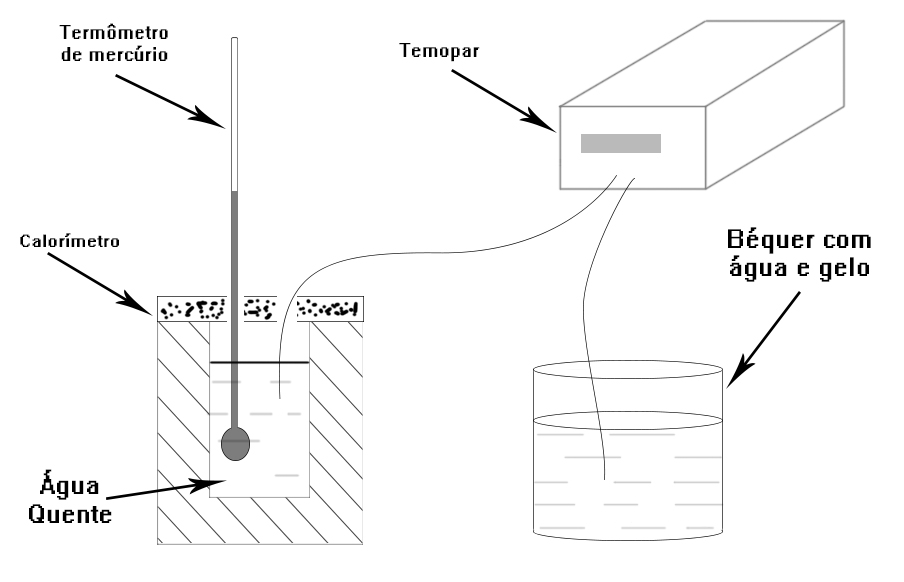
\includegraphics[scale=0.3]{Fig6a2.jpg}
\caption{Montagem experimental para a calibração do termopar.}
\label{exptermopar}
\end{figure}


\subsubsection{Constante de tempo de um calorímetro}
szkjdgb

\subsubsection{Capacidade térmica de um calorímetro}
siough



\subsection{Dados Obtidos}




\section{Análise dos Resultados e Discussões}

\subsection{Regressão linear}

\subsection{Significado físico do coeficiente angular}



\section{Conclusões}


\section{Bibliografia}

\end{document}

